\section{Diagrams}

\subsection{Simple Flowchart}

\tikzstyle{startstop} = [rectangle, rounded corners, minimum width=3cm, minimum height=1cm,text centered, draw=black, fill=red!30]
\tikzstyle{process} = [rectangle, minimum width=3cm, minimum height=1cm, text centered, draw=black, fill=orange!30]
\tikzstyle{decision} = [diamond, minimum width=3cm, minimum height=1cm, text centered, draw=black, fill=green!30]
\tikzstyle{arrow} = [thick,->,>=stealth]
\begin{center}
\begin{tikzpicture}[node distance=2cm]
    \node (start) [startstop] {Start};
    \node (process1) [process, below of=start] {Process 1};
    \node (decision1) [decision, below of=process1, yshift=-1cm] {Decision 1};
    \node (process2a) [process, below of=decision1, yshift=-1cm] {Process 2a};
    \node (process2b) [process, right of=decision1, xshift=3cm] {Process 2b};
    \node (stop) [startstop, below of=process2a] {Stop};

    \draw [arrow] (start) -- (process1);
    \draw [arrow] (process1) -- (decision1);
    \draw [arrow] (decision1) -- node[anchor=east] {Yes} (process2a);
    \draw [arrow] (decision1) -- node[anchor=south] {No} (process2b);
    \draw [arrow] (process2a) -- (stop);
    \draw [arrow] (process2b.east) -- ++(1,0) |- (process1.east);
\end{tikzpicture}
\end{center}


\subsection{Decision Tree}
\begin{center}
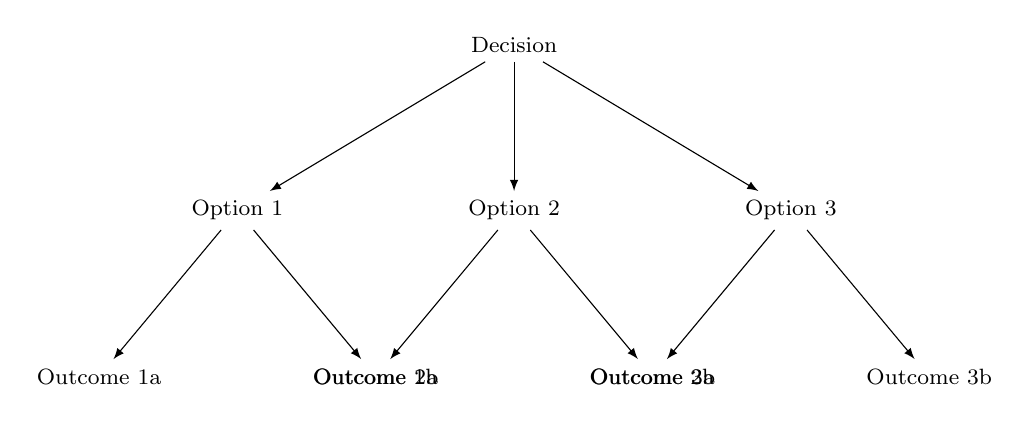
\begin{tikzpicture}[
    edge from parent/.style={draw, -latex},
    sibling distance=10em, level distance=6em,
    every node/.style={font=\footnotesize}]
    
    \node {Decision}
        child { node {Option 1}
            child { node {Outcome 1a} }
            child { node {Outcome 1b} }
        }
        child { node {Option 2}
            child { node {Outcome 2a} }
            child { node {Outcome 2b} }
        }
        child { node {Option 3}
            child { node {Outcome 3a} }
            child { node {Outcome 3b} }
        };
\end{tikzpicture}
\end{center}

\subsection{Data Flow Diagram}
\tikzstyle{process} = [rectangle, minimum width=3cm, minimum height=1cm, text centered, draw=black, fill=orange!30]
\tikzstyle{data} = [trapezium, trapezium left angle=70, trapezium right angle=110, minimum width=2cm, minimum height=1cm, text centered, draw=black, fill=yellow!30]
\tikzstyle{arrow} = [thick,->,>=stealth]

\begin{tikzpicture}[node distance=1.5cm]
    \node (input) [data] {Input Data};
    \node (process1) [process, right of=input, xshift=3cm] {Process 1};
    \node (data) [data, below of=process1, yshift=-1cm] {Stored Data};
    \node (process2) [process, right of=process1, xshift=3cm] {Process 2};
    \node (output) [data, right of=process2, xshift=3cm] {Output Data};

    \draw [arrow] (input) -- (process1);
    \draw [arrow] (process1) -- (data);
    \draw [arrow] (data) -- (process2);
    \draw [arrow] (process2) -- (output);
    \draw [arrow] (data.north) -- ++(0,1) -| (process2.south);
\end{tikzpicture}


\subsection{Class Diagram}
\begin{center}
\begin{tikzpicture}[
    class/.style={
        rectangle,
        draw=black,
        fill=blue!20,
        text centered,
        minimum width=3cm,
        minimum height=2cm
    },
    relation/.style={
        -{stealth[open]},
        thick
    },
    aggregation/.style={
        -{diamond[open]},
        thick
    },
    composition/.style={
        -{diamond[fill=black]},
        thick
    },
    generalization/.style={
        -{stealth[open]},
        thick
    }
]

\node[class] (classA) {
    \begin{tabular}{c}
    \textbf{Class A} \\
    \hline
    +attribute1 \\
    +attribute2
    \end{tabular}
};
\node[class] (classB) [below left=of classA] {
    \begin{tabular}{c}
    \textbf{Class B} \\
    \hline
    +attribute3 \\
    +attribute4
    \end{tabular}
};
\node[class] (classC) [below right=of classA] {
    \begin{tabular}{c}
    \textbf{Class C} \\
    \hline
    +attribute5 \\
    +attribute6
    \end{tabular}
};

\draw[relation] (classA) -- (classB) node[midway, fill=white] {1..*};
\draw[aggregation] (classA) -- (classC) node[midway, fill=white] {1};
\draw[composition] (classB) -- (classC) node[midway, fill=white] {0..1};

\end{tikzpicture}
\end{center}